\documentclass{article} % For LaTeX2e
\usepackage{iclr2017_conference,times}
\usepackage{hyperref}
\usepackage{url}
% \usepackage[dvips]{graphicx}

% from Exploring Policy Rep
\usepackage[utf8]{inputenc}
\usepackage{hyperref}
\usepackage{amssymb}
\usepackage{amsmath}
\usepackage{newclude}
\usepackage[normalem]{ulem}
\usepackage{dsfont}

\usepackage{subfigure}
\newcommand{\R}{\mathbb{R}}
\usepackage{changepage}
\usepackage{graphicx}

\usepackage{pdfpages}

\usepackage{cancel}

\title{Stochastic Neural Networks for \\Hierarchical Reinforcement Learning}


\author{Carlos Florensa, Yan Duan \& Pieter Abbeel \\
Department of Electrical Engineering and Computer Sciences\\
UC Berkeley\\
\texttt{\{florensa,dementrock,pabbeel\}@berkeley.edu}
}

% The \author macro works with any number of authors. There are two commands
% used to separate the names and addresses of multiple authors: \And and \AND.
%
% Using \And between authors leaves it to \LaTeX{} to determine where to break
% the lines. Using \AND forces a linebreak at that point. So, if \LaTeX{}
% puts 3 of 4 authors names on the first line, and the last on the second
% line, try using \AND instead of \And before the third author name.

\newcommand{\fix}{\marginpar{FIX}}
\newcommand{\new}{\marginpar{NEW}}

%\iclrfinalcopy % Uncomment for camera-ready version

\begin{document}
	
	\maketitle

\begin{abstract}

Many practical problems in Reinforcement Learning (RL) only have a high level reward signal. This includes all tasks where a reward is only received when reaching a certain goal, even if many coordinated actions need to be taken before. Therefore these tasks have a \textit{sparse reward} and are considered some of the hardest in the field. To tackle them the two main approaches are reward shaping (eg. with some intrinsic motivation for exploration bonus) or using hand-engineered sequences of actions that allow to hierarchize the task and take high level actions (\textit{skills}, \textit{macro-actions} or \textit{options}). The first method can be completely unsupervised but the learning for one specific goal is difficult to re-use for another goal, even if the underlying dynamics are the same. The second method grants better re-use of skills but the prior knowledge needed to design the \textit{macro-actions} is undesired. In the present work we combine the best of both worlds to obtain \textit{skills} in a completely unsupervised fashion via a pre-training step and then use them to solve the actual task. We prove that a good "span of skills" can be learned using Stochastic Neural Networks (SNN) given their extra expressive power. The property of yielding different solutions to the MDP at the end of training (instead of a single one as most RL algorithms) is very interesting and we outline other uses in domain adaptation and bad local minima avoidance.
\end{abstract}

\section{Introduction}

% - What is the problem?
% - Why is it interesting and important?
% - Why is it hard? (E.g., why do naive approaches fail?) OK
% - Why hasn't it been solved before? (Or, what's wrong with previous proposed solutions? How does mine differ?)
% - What are the key components of my approach and results? Also include any specific limitations.


Recent advances in Deep Reinforcement Learning allow to train agents with super-human performance in tasks with discrete action-space like Go \cite{2016go} or some Atari games \cite{mnih2015human}. Nevertheless, many challenges remain in the continuous state-action environments, and in particular the problem of tasks with sparse reward is even more acute in the continuous case. In robotics, tasks like navigation or manipulation only have a natural reward in the goal position, and it is often hard to provide constant supervision along the trajectories with a cost function tailored to the task [cite IRL litterature?]. The main difficulty is that a sequence of well coordinated actions, producing a purposeful motion, is required to get any reward signal. Hence, as has been reported in the recent benchmark for continuous control tasks \cite{yuan2015}, it is very unlikely that the usual $\epsilon$-Greedy or Boltzmann exploration [ref] or adding Gaussian noise to the controls for policy gradient algorithms [TRPO], will yield a trajectory providing any feedback. 

To tackle this issue/challenge there are two main approaches and in this paper we will combine the best of both. One consists in providing an exploration bonus to the agent so that, despite not getting to the goal, it is still pushed to explore unseen regions that could potentially contain the extrinsic reward. In discrete MDPs this intrinsic reward may take many forms, from the simplest based on state-counting (rewarding each state inversely proportional to a function of its visitation counts) [refm, DM, simHash] to information theory-based like surprisal [ ref!! ]. In the continuous domain, VIME uses variatinal inference in Bayesian neural networks to incentivize exploration.

it is common to provide a specific abstraction of the problem.

\section{Methodology}

\subsection{Preliminaries}
\begin{itemize}
    \item describe MDP?
    \item introduce learning agent-centric skills
    \item introduce "intrinsic rewards" (COM speed)
\end{itemize}

Words from ICLR call for papers:
- Unsupervised
- Representation learning for planning and reinforcement learning
- Hierarchical models
- application to robotics

\subsection{Stochastic Neural Networks}

\begin{itemize}
    \item To solve continuous MDPS with Policy Gradient methods \citep{peters2008reinforcement}, a stochastic policy is required [appart if you do DDPG?]. The usual is to use a deterministic neural network to parametrize the mean $\mu(s_t)$ and variance $\Sigma(s_t)$ of a Gaussian distribution, from where the next action $a_{t+1}$ is sampled. From the re-parametrization trick perspective \citep{look at SVG paper or DeepMind-modulate}, this corresponds to simply having a linear combination of normal noise at the output of the neural network:
    \begin{equation}
        a_{t+1} = \mu_{\theta}(s_t) +\epsilon \Sigma_\theta(s_t), ~~~~ \epsilon \sim \mathbb{N}(0,I)
    \end{equation}
    \item Hence, despite the arbitrary expresiveness of the neural networks, the noise addition process is very restricted, with two major drawbacks. On one hand the exploration is limited and this process will not perform well for continuous sparse hierarchical tasks. 
    
    On the other hand the policy will be unimodal by construction!
\end{itemize}
The usual Stochastic Feedforward Neural Networks were first described by \citet{tang2013sfnn}

\subsection{Bilinear Integration of latents}

\subsection{Entropy Penalty to encourage skill diversity}

\section{Experiments}

\subsection{Pre-training task: Learning to move}
Our pre-training task is as unuspervised as it can be: 

\subsection{Hierarchical task: Maze Navigation}

\begin{figure}[h!]
	\centering
	\subfigure[Reward function of the point MDP]{
		\centering
		\label{fig:reward_func}
		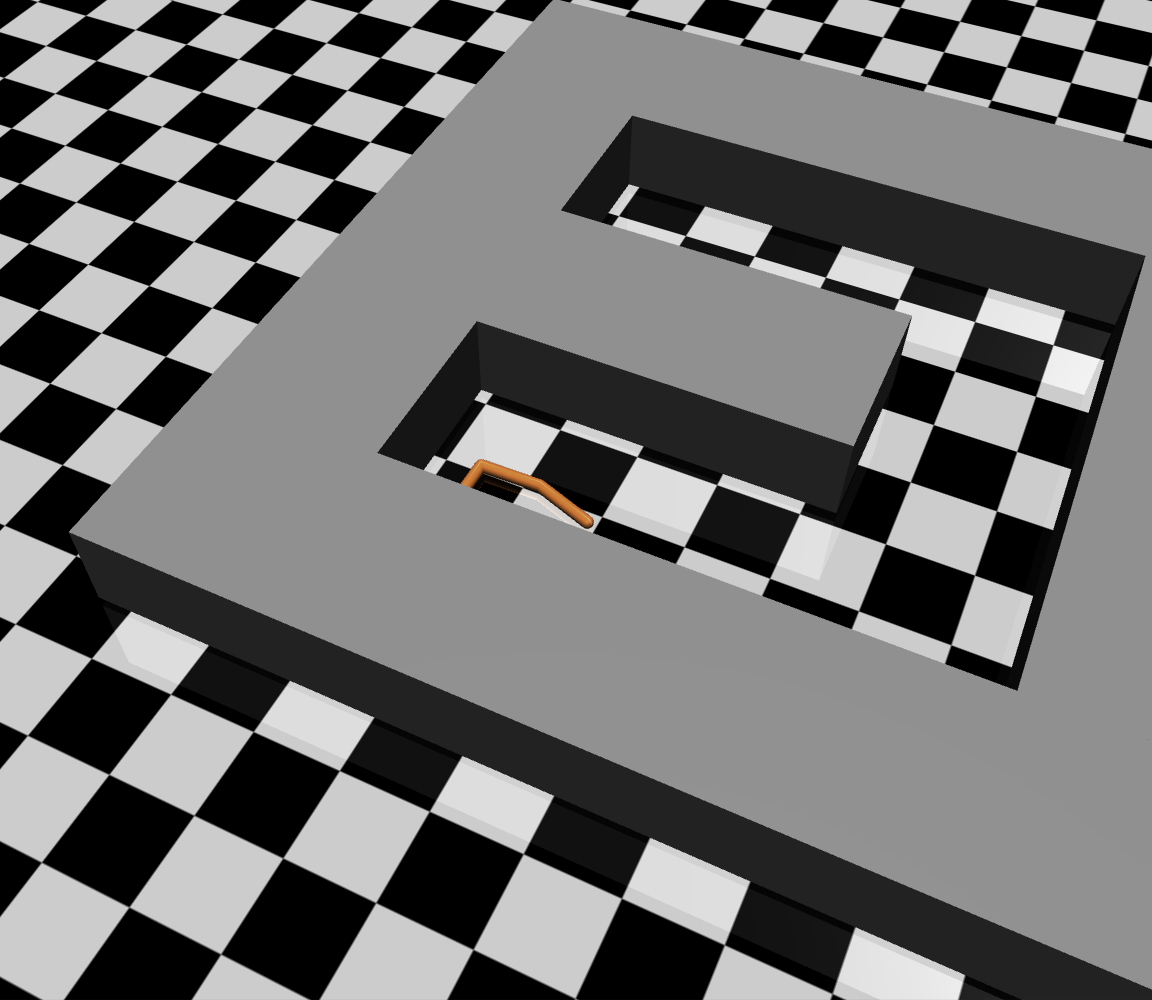
\includegraphics[width = 0.45\textwidth]{Figures/Maze0.png}
	}
	\subfigure[An example of non-multimodal without MIreward nor hallucinations]{
		\centering
		\label{fig:no_multimode_withoutMI}
		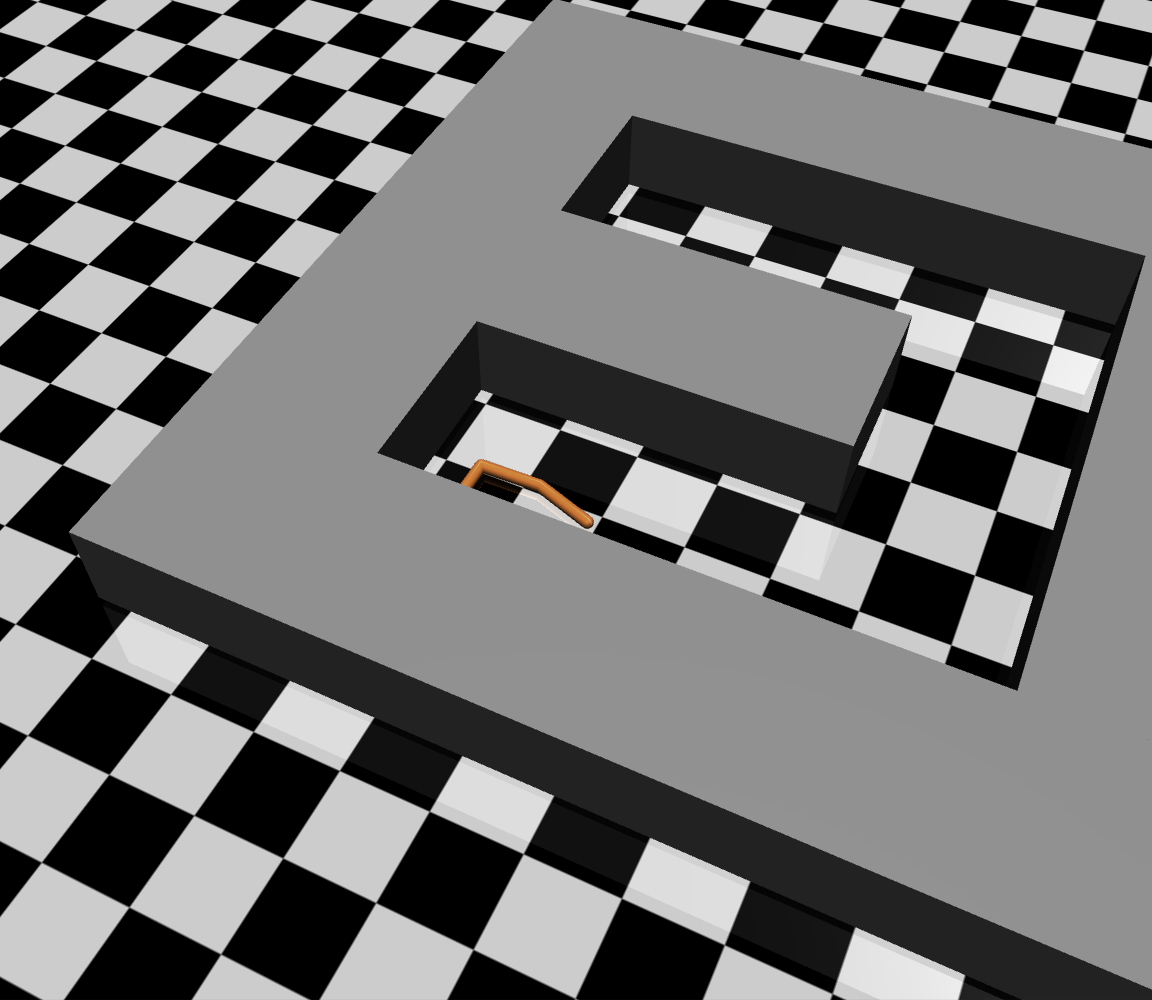
\includegraphics[width = 0.45\textwidth]{Figures/Maze0.png}
	}
	\caption{Examples of performance and final policies learned by the SNN on the 2D and 4 modes point-MDP, with 1 latent Bernoulli variables.}
	\label{fig:snn_multimodal_MI}
\end{figure}

\section{Results}

\section{Conclusions}

\subsubsection*{Acknowledgments}

Use unnumbered third level headings for the acknowledgments. All
acknowledgments, including those to funding agencies, go at the end of the paper.

\bibliography{ref}
\bibliographystyle{iclr2017_conference}

\end{document}
